\documentclass[aspectratio=169,11pt]{beamer}
\usepackage[T1]{fontenc}
\usepackage[utf8]{inputenc}
\usepackage{lmodern}
\usepackage{amsmath,amssymb}
\usepackage{booktabs}\usepackage{array}
\usepackage{tikz}
\usepackage{pgfplots}
\pgfplotsset{compat=1.17}
\usetikzlibrary{arrows.meta,positioning,calc}

% ---------- look ----------
\definecolor{accent}{HTML}{14325A}
\definecolor{hl}{HTML}{C8501E}
\definecolor{soft}{HTML}{EEF2F7}
\setbeamertemplate{navigation symbols}{}
\setbeamercolor{background canvas}{bg=white}
\setbeamercolor{normal text}{fg=black!85}
\setbeamercolor{structure}{fg=accent}
\setbeamersize{text margin left=0.6cm,text margin right=0.6cm}
\setbeamertemplate{itemize items}[circle]
\setbeamercolor{itemize item}{fg=hl}
\setbeamerfont{itemize/enumerate body}{size=\small}
\setbeamerfont{itemize/enumerate subbody}{size=\footnotesize}
\setlength{\leftmargini}{1.1em}
\setbeamertemplate{frametitle}{%
  \vskip0.18cm
  \begin{beamercolorbox}[wd=\paperwidth,leftskip=0.6cm,rightskip=0.6cm,sep=0pt]{frametitle}
    \parbox{\dimexpr\paperwidth-1.2cm}{\raggedright\bfseries\large\color{accent}\insertframetitle\par}
    \vskip1pt{\color{hl}\rule{2.2cm}{1.4pt}}
  \end{beamercolorbox}\vskip-0.05cm}
\setbeamertemplate{footline}{%
  \leavevmode\hbox to\paperwidth{\hspace*{0.6cm}\color{black!55}\tiny Tee, Xinrui, Fong How \textbullet\ Missing fourth basis in dimension six\hfill\insertframenumber\hspace*{0.6cm}}\vskip0.18cm}

% ---------- status tags ----------
\newcommand{\tg}[2]{{\setlength{\fboxsep}{1.4pt}\colorbox{#1}{\textcolor{white}{\sffamily\bfseries\scriptsize\,#2\,}}}}
\definecolor{cProved}{HTML}{1B7F3B}
\definecolor{cLean}{HTML}{0E7C86}
\definecolor{cCert}{HTML}{1F4FB5}
\definecolor{cComp}{HTML}{5B6B7F}
\definecolor{cNum}{HTML}{C77700}
\definecolor{cCited}{HTML}{7A7A7A}
\definecolor{cCond}{HTML}{7B3FA0}
\definecolor{cOpen}{HTML}{B3262B}
\newcommand{\Tproved}{\tg{cProved}{proved here}}
\newcommand{\Tlean}{\tg{cLean}{Lean-checked, as reported}}
\newcommand{\Tcert}{\tg{cCert}{interval-certified}}
\newcommand{\Tcomp}{\tg{cComp}{computed}}
\newcommand{\Tnum}{\tg{cNum}{numerical only}}
\newcommand{\Tcited}{\tg{cCited}{cited}}
\newcommand{\Tcond}{\tg{cCond}{conditional}}
\newcommand{\Topen}{\tg{cOpen}{conjecture / open}}
\definecolor{cRep}{HTML}{3D6B3D}
\newcommand{\Trep}{\tg{cRep}{reported, not re-run}}
\newcommand{\Trepn}{{\setlength{\fboxsep}{1.4pt}\colorbox{cRep}{\textcolor{white}{\sffamily\bfseries\tiny\,reported, not re-run\,}}}}

% ---------- notation ----------
\newcommand{\C}{\mathbb{C}}
\newcommand{\ip}[2]{\langle #1,#2\rangle}
\newcommand{\abs}[1]{\lvert #1\rvert}
\newcommand{\norm}[1]{\lVert #1\rVert}
\newcommand{\cstar}{c_\ast}
\newcommand{\hcube}[1]{#1^{\circ3}}

\title{The missing fourth basis in dimension six}
\author{Tee}
\date{}

\begin{document}

% ======================= TITLE =======================
\begin{frame}[plain]
\vspace*{0.5cm}
\begin{center}
{\bfseries\LARGE\color{accent} The missing fourth basis in dimension six:\\[2pt] what is verified, how far away it is,\\[2pt] and how to see it\par}
\vspace{0.35cm}
{\color{hl}\rule{3cm}{1.6pt}}\\[0.4cm]
{\large Ren Jie Tee (UC Berkeley), Xinrui, Raymond Fong How (Georgia Tech)\par}
\vspace{0.35cm}
{\normalsize Caltech $\times$ SAIR Mathathon, Problem 124\\
Track: Computation/Applied Mathematics\par}
\vspace{0.5cm}
{\footnotesize Every claim carries a status tag:\\[3pt] \Tproved\ \Tlean\ \Tcert\ \Tcomp\ \Tnum\ \Tcited\ \Tcond\ \Topen\ \Trep}
\end{center}
\end{frame}

\setcounter{framenumber}{0}
% ======================= 1 =======================
\begin{frame}{In dimension six, three mutually unbiased bases are easy to build and a fourth has never been found}
\begin{columns}[T]
\begin{column}{0.47\textwidth}
\small
\begin{itemize}\setlength\itemsep{4pt}
\item Bases $e,f$ of $\C^6$ are \emph{unbiased}: $\abs{\ip{e_i}{f_j}}^2=\tfrac16$ for all $i,j$.
\item Zauner (1999) conjectured at most three exist, $N(6)=3$. \Tcited
\item Three 2026 computer-assisted preprints claim it. \Tcited
\item Dimension ten, the next case $2\times$ prime: open. \Tcited
\end{itemize}
\vspace{0.1cm}
\footnotesize We ask: how do we know, by how much, and what would one see in a laboratory?
\end{column}
\begin{column}{0.53\textwidth}
\centering
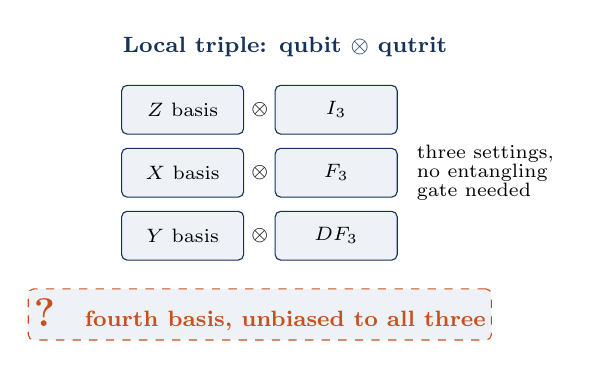
\begin{tikzpicture}[font=\scriptsize,
  bx/.style={draw=accent,fill=soft,rounded corners=2pt,minimum height=0.62cm,minimum width=1.55cm,inner sep=2pt}]
 \node[font=\footnotesize\bfseries,color=accent] at (2.1,3.05) {Local triple: qubit $\otimes$ qutrit};
 \node[bx] (a1) at (0.8,2.25) {$Z$ basis};  \node at (1.78,2.25) {$\otimes$}; \node[bx] (b1) at (2.75,2.25) {$I_3$};
 \node[bx] (a2) at (0.8,1.45) {$X$ basis};  \node at (1.78,1.45) {$\otimes$}; \node[bx] (b2) at (2.75,1.45) {$F_3$};
 \node[bx] (a3) at (0.8,0.65) {$Y$ basis};  \node at (1.78,0.65) {$\otimes$}; \node[bx] (b3) at (2.75,0.65) {$DF_3$};
 \node[right,align=left] at (3.65,1.45) {three settings,\\[-1pt]no entangling\\[-1pt]gate needed};
 \node[bx,dashed,draw=hl,minimum width=3.9cm,minimum height=0.65cm] (q) at (1.78,-0.35) {\Large\bfseries\color{hl}?\ \ \footnotesize fourth basis, unbiased to all three};
\end{tikzpicture}
\end{column}
\end{columns}
\end{frame}

% ======================= 2 =======================
\begin{frame}{Three 2026 computer proofs say $N(6)=3$, and none is formally verified end to end}
\centering\footnotesize
\renewcommand{\arraystretch}{1.2}
\begin{tabular}{@{}>{\raggedright\arraybackslash}p{1.6cm}>{\raggedright\arraybackslash}p{3.7cm}>{\raggedright\arraybackslash}p{3.5cm}>{\raggedright\arraybackslash}p{4.2cm}@{}}
\toprule
 & OpenAI & Jaswal & C\'ardenes Wuttig, Tindall\\
\midrule
Method & 249,878 seed centers, graph search for two further bases & same method, re-implemented & 2,775 balls plus one at the Fourier matrix\\
Arithmetic & binary64 with margins & binary64 intervals & Arb balls, Julia checker\\
Lean & proves $N(6)\le5$ only & none & certificate $\Rightarrow$ no four MUBs; numbers outside Lean\\
\bottomrule
\end{tabular}\\[0.15cm]
\raggedright\small\hspace{0.2cm}\Tcited\ Shared ancestry and trusted base; all three AI-assisted by their authors' account. Our map of Jaswal rests on a summary. Reading is not verification: we did not check their mathematics.\\[0.2cm]
\begin{beamercolorbox}[wd=\textwidth,sep=4pt,rounded=true]{soft}
\scriptsize\textbf{Status tags used in this talk:}\ \Tproved\ \Tlean\ \Tcert\ \Tcomp\ \Tnum\ \Tcited\ \Tcond\ \Topen\ \Trep\\[2pt]
\textcolor{black!70}{proved here by hand; Lean built by a teammate; ball arithmetic or exact certificate; computed (range stated); local minimisation only; literature; depends on a stated hypothesis; unproved; run by a teammate, not re-run by us.}
\end{beamercolorbox}
\end{frame}

% ======================= 3 =======================
\begin{frame}{We reran what an outsider can rerun: the checker catches 17 of 26 corruptions, and the rebuilt parts match bit for bit}
\small
\begin{itemize}\setlength\itemsep{4pt}
\item OpenAI's record checker passes unmodified; counts match the preprint. \Tcomp
\item \textbf{Mutation test:} 26 small corruptions of the saved records, 17 detected, 9 missed (2 harmless, 7 scope gaps: stored values are only range-checked). Run twice, identical verdicts. \Tcomp
\item \textbf{Partial rebuild} (seed cover, two stage-C batches): bit-identical, on the preprint's own toolchain, so independence is weak. \Tcomp
\item \textbf{Full native rerun} (workstream C, not re-run by us): 100 invocations, 8 principal files byte-identical, 27,188 root records re-certified in 128-bit Arb. \Trep
\item Fourier pair $\{I,F_6\}$ redone: $156\to48\to16\to0$, given the cited count 156. \Tcond
\end{itemize}
\vspace{0.1cm}
\begin{beamercolorbox}[wd=\textwidth,sep=4pt,rounded=true]{soft}
\footnotesize A miss is a statement about the checker, not a flaw in the theorem. Byte agreement shows reproducibility, not that the covering lemmas are right.
\end{beamercolorbox}
\end{frame}

% ======================= 4 =======================
\begin{frame}{We can prove structure for order-six Hadamard matrices, but the universal step toward $N(6)=3$ is still open}
\centering
\vspace{0.2cm}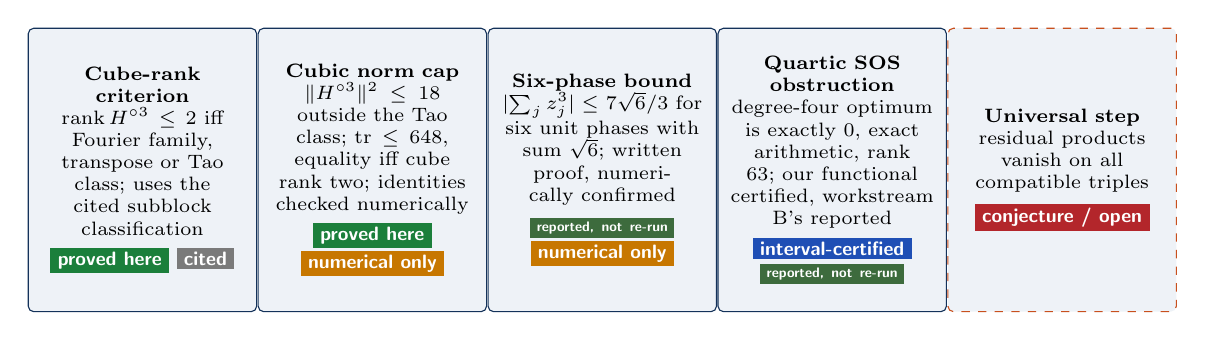
\begin{tikzpicture}[font=\scriptsize,
  bx/.style={draw=accent,fill=soft,rounded corners=2pt,text width=2.62cm,align=center,minimum height=3.6cm,inner sep=4pt}]
 \node[bx] (a) at (0,0) {\textbf{Cube-rank criterion}\\ $\operatorname{rank}\hcube{H}\le2$ iff Fourier family, transpose or Tao class; uses the cited subblock classification\\[3pt]\Tproved\ \Tcited};
 \node[bx] (b) at (2.92,0) {\textbf{Cubic norm cap}\\ $\norm{\hcube{H}}^2\le18$ outside the Tao class; $\operatorname{tr}\le648$, equality iff cube rank two; identities checked numerically\\[3pt]\Tproved\ \Tnum};
 \node[bx] (c) at (5.84,0) {\textbf{Six-phase bound}\\ $\abs{\sum_j z_j^3}\le7\sqrt6/3$ for six unit phases with sum $\sqrt6$; written proof, numerically confirmed\\[3pt]\Trepn\ \Tnum};
 \node[bx] (d) at (8.76,0) {\textbf{Quartic SOS obstruction}\\ degree-four optimum is exactly $0$, exact arithmetic, rank $63$; our functional certified, workstream B's reported\\[3pt]\Tcert\ \Trepn};
 \node[bx,dashed,draw=hl] (e) at (11.68,0) {\textbf{Universal step}\\ residual products vanish on all compatible triples\\[3pt]\Topen};
\end{tikzpicture}\\[0.25cm]
\raggedright\small
\hspace{0.2cm}Equality in the trace bound holds iff the cube rank is two; ``norm $18$ implies cube rank two'' is \Topen. Nothing here yet bounds the number of MUBs.
\end{frame}

% ======================= 5 =======================
\begin{frame}{No pure state hides from the local triple: its energy is above $0.0384999$, which is 99.3\% of the exact minimum}
\small
$E(\psi)=\sum_{18\text{ outcomes}}(p-\tfrac16)^2$, and $E=0$ exactly for a state unbiased to all three bases.\\[0.1cm]
\centering
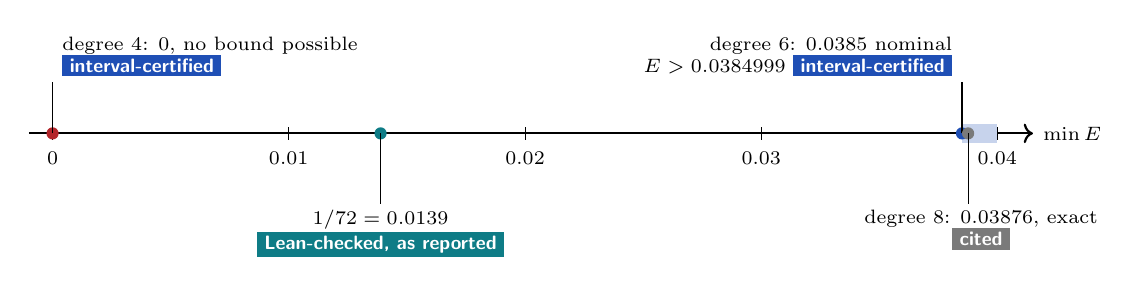
\begin{tikzpicture}[x=300cm,y=1cm,font=\scriptsize]
 \draw[->,thick] (-0.001,0)--(0.0415,0) node[right] {$\min E$};
 \foreach \t in {0,0.01,0.02,0.03,0.04} {\draw (\t,0.08)--(\t,-0.08) node[below=1pt] {\t};}
 \fill[cCert!25] (0.0385,-0.12) rectangle (0.04,0.12);
 \fill[cOpen] (0,0) circle (2.2pt);
 \draw (0,0)--(0,0.65); \node[above right,align=left] at (0,0.6) {degree 4: $0$, no bound possible\\ \Tcert};
 \fill[cLean] (0.013889,0) circle (2.2pt);
 \draw (0.013889,0)--(0.013889,-0.9); \node[below,align=center] at (0.013889,-0.85) {$1/72=0.0139$\\ \Tlean};
 \fill[cCert] (0.0385,0) circle (2.2pt);
 \draw (0.0385,0)--(0.0385,0.65); \node[above left,align=right] at (0.0385,0.6) {degree 6: $0.0385$ nominal\\ $E>0.0384999$ \Tcert};
 \fill[cCited] (0.0387628,0) circle (2.2pt);
 \draw (0.0387628,0)--(0.0387628,-0.9); \node[below,align=center] at (0.0393,-0.85) {degree 8: $0.03876$, exact\\ \Tcited};
\end{tikzpicture}\\[0.25cm]
\raggedright\footnotesize
\hspace{0.2cm}The exact value $(4-\sqrt6)/40$ is prior work of Erlwein. Ours is an independent certificate at lower degree, not a new bound.\\[2pt]
\hspace{0.2cm}Same method: $E>0.0234999$ for the second product triple and for all $16$ triples containing $I$ and $F_6$, given the classical count $156$. \Tcert
\end{frame}

% ======================= 6 =======================
\begin{frame}{A $10^{-7}$ threshold accepted two near-misses, so ``found numerically'' is not ``proved''}
\centering\footnotesize
\renewcommand{\arraystretch}{1.35}
\begin{tabular}{@{}lcccc@{}}
\toprule
Shape & 2008 hit rate & misfit $\mu=\norm{r}_2$ at strict local min & 2008 $F=\mu^2/36$ there & 2008 threshold\\
\midrule
$\{5,4,4,1\}_6$ & 0.74\% & $1.02497683851953\times10^{-3}$ & $2.9\times10^{-8}$ & $10^{-7}$\\
$\{5,5,3,1\}_6$ & 1.47\% & $7.32788656303688\times10^{-4}$ & $1.5\times10^{-8}$ & $10^{-7}$\\
\bottomrule
\end{tabular}\\[0.1cm]
\raggedright\small
\hspace{0.2cm}\Tcert\ Certified strict local minima with nonzero misfit that pass the 2008 acceptance test, so the two entries become \emph{undecided, not refuted}. We do not prove the shapes empty.
\begin{itemize}\setlength\itemsep{3pt}
\item Converse: $\{5,3,3,3\}_6$ exists, yet one start in 20,000 finds it. \Tcomp
\item Thirteen shapes of the 2008 table remain undecided. \Topen
\end{itemize}
\end{frame}

% ======================= 7 =======================
\begin{frame}{One certified vector bound forces every fourth basis to be far from unbiased, farther than explicit quadruples}
\small
\begin{beamercolorbox}[wd=\textwidth,sep=3pt,rounded=true]{soft}
\centering\footnotesize\vspace{-2pt}
$\displaystyle\sqrt p\le\tfrac1{\sqrt6}+\tfrac{\sqrt6}2\bigl(p-\tfrac16\bigr)-\cstar\bigl(p-\tfrac16\bigr)^2$ on $[0,1]$, $\cstar=\tfrac{3\sqrt6}{(\sqrt6+1)^2}$ \Tproved
\end{beamercolorbox}
\footnotesize
\vspace{0.05cm}
If $E\ge\gamma$ on all unit vectors, any fourth basis has bias $\ge\sqrt{\gamma/18}$ and game loss $\ge\cstar\gamma/72$. \Tproved\ With $E>0.0384999$ (canonical triple):
\vspace{0.05cm}

\centering
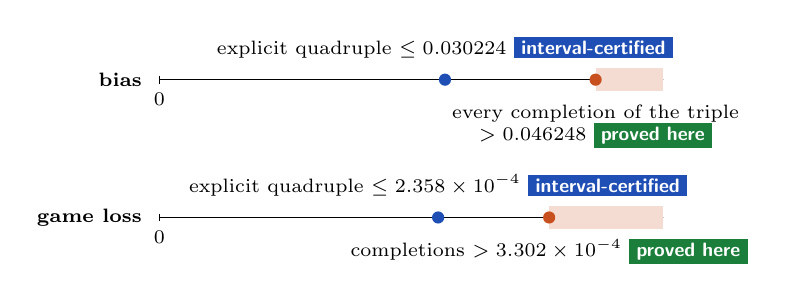
\begin{tikzpicture}[font=\scriptsize]
 \node[anchor=east] at (-0.1,1.75) {\textbf{bias}};
 \draw[->] (0,1.75)--(6.4,1.75);
 \fill[hl!20] (5.54,1.6) rectangle (6.4,1.9);
 \draw (0,1.8)--(0,1.7) node[below=0pt] {0};
 \fill[cCert] (3.627,1.75) circle (2.2pt); \node[above,align=center] at (3.627,1.9) {explicit quadruple $\le0.030224$ \Tcert};
 \fill[hl] (5.54,1.75) circle (2.2pt); \node[below,align=center] at (5.54,1.55) {every completion of the triple\\ $>0.046248$ \Tproved};
 \node[anchor=east] at (-0.1,0) {\textbf{game loss}};
 \draw[->] (0,0)--(6.4,0);
 \fill[hl!20] (4.95,-0.15) rectangle (6.4,0.15);
 \draw (0,0.05)--(0,-0.05) node[below=0pt] {0};
 \fill[cCert] (3.54,0) circle (2.2pt); \node[above,align=center] at (3.54,0.15) {explicit quadruple $\le2.358\times10^{-4}$ \Tcert};
 \fill[hl] (4.95,0) circle (2.2pt); \node[below,align=center] at (4.95,-0.15) {completions $>3.302\times10^{-4}$ \Tproved};
\end{tikzpicture}\\[0.1cm]
\raggedright\hspace{0.2cm}\textbf{Design lesson:} the best approximate quadruples are not completions of the perfect local triple. The two explicit quadruples minimise bias and maximise the game score. For the second product triple the bias lesson holds and the game comparison is inconclusive.
\end{frame}

% ======================= 8 =======================
\begin{frame}{Hide and seek is a theorem: with 1,936 shots per setting, a collision test flags every pure state as not white noise}
\begin{columns}[T]
\begin{column}{0.46\textwidth}
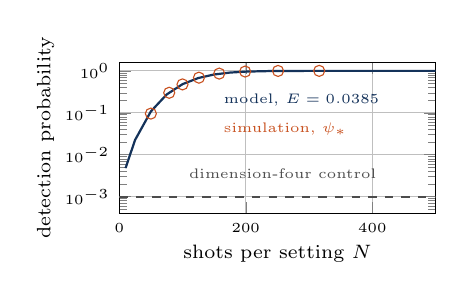
\begin{tikzpicture}
\begin{axis}[width=5.6cm,height=3.5cm,xmin=0,xmax=500,ymode=log,ymin=4e-4,ymax=1.6,
  xlabel={shots per setting $N$},ylabel={detection probability},grid=major,
  tick label style={font=\tiny},label style={font=\scriptsize},xlabel style={yshift=2pt},ylabel style={yshift=-3pt}]
\addplot[thick,accent] coordinates {(10,0.0048) (25,0.0224) (50,0.1078) (75,0.2733) (100,0.4812) (125,0.6751)
  (150,0.8197) (175,0.9102) (200,0.9594) (239,0.9901) (250,0.9935) (300,0.9992) (350,0.9999) (400,1.0) (500,1.0)};
\addplot[only marks,mark=o,hl] coordinates {(50,0.0957) (79,0.30025) (100,0.47565) (126,0.6884) (158,0.8604)
  (199,0.9628) (251,0.9957) (316,0.9998)};
\addplot[thick,dashed,black!70] coordinates {(0,0.001) (500,0.001)};
\node[font=\tiny,anchor=west,text=accent] at (axis cs:150,0.2) {model, $E=0.0385$};
\node[font=\tiny,anchor=west,text=hl] at (axis cs:150,0.04) {simulation, $\psi_\ast$};
\node[font=\tiny,anchor=south west,text=black!70] at (axis cs:95,0.0016) {dimension-four control};
\end{axis}
\end{tikzpicture}\\[2pt]
\centering\scriptsize
\renewcommand{\arraystretch}{1.1}
\begin{tabular}{@{}lcccc@{}}
\toprule
two-qubit error & 0 & 0.1\% & 1\% & 10\%\\
total shots & 589 & 594 & 646 & 1,500\\
\bottomrule
\end{tabular}\\[1pt]
{\tiny 50\% detection at five-sigma false alarm, large-sample model \Tcomp}
\end{column}
\begin{column}{0.54\textwidth}
\begin{itemize}\scriptsize\setlength\itemsep{3pt}
\item \textbf{Theorem.} $T$, the collision estimator, is unbiased for $E$; Pearson's $X^2=15+6(N-1)T$ exactly. With $N=1{,}936$ every pure state is flagged with probability $\ge95\%$, false alarm $\le0.1\%$; $N=5{,}142$ gives $99\%$ and $0.1\%$. \Tproved\ from certified inputs
\item \textbf{Rule of thumb:} $239$ shots ($99\%$, $0.1\%$), an approximation checked by simulation, optimistic below $N=100$. \Tcomp
\item \textbf{Purity witness:} exactly uniform statistics force the largest eigenvalue to be at most $0.8232$. \Tproved
\item \textbf{Not new:} the test is the classical collision test (Goldreich--Ron, Paninski); strongly unextendible triples as witnesses: Grassl, McNulty, Mi\v{s}ta, Paterek (2017). \Tcited\ \textbf{Ours:} feeding it the certified energy gap.
\item The game needs $9.37\times10^7$ rounds, a different question. Dimension four: never caught. No hardware run.
\end{itemize}
\end{column}
\end{columns}
\end{frame}

% ======================= 9 =======================
\begin{frame}{Dimension ten with the same method: 34,940 certified cyclic roots funnel down to 1,136 candidate bases, and none extends}
\centering
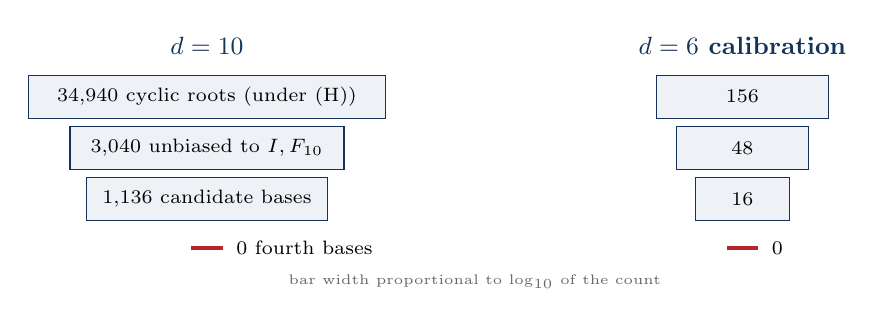
\begin{tikzpicture}[x=1cm,y=1cm,font=\scriptsize,
  st/.style={draw=accent,fill=soft,minimum height=0.55cm,inner sep=1pt}]
  \node[font=\small\bfseries,color=accent] at (2.2,0.95) {$d=10$};
  \node[st,minimum width=4.54cm] at (2.2,0.3) {34,940 cyclic roots (under (H))};
  \node[st,minimum width=3.48cm] at (2.2,-0.35) {3,040 unbiased to $I,F_{10}$};
  \node[st,minimum width=3.06cm] at (2.2,-1.0) {1,136 candidate bases};
  \draw[very thick,cOpen] (2.0,-1.62)--(2.4,-1.62); \node[right] at (2.45,-1.62) {0 fourth bases};
  \node[font=\small\bfseries,color=accent] at (9.0,0.95) {$d=6$ calibration};
  \node[st,minimum width=2.19cm] at (9.0,0.3) {156};
  \node[st,minimum width=1.68cm] at (9.0,-0.35) {48};
  \node[st,minimum width=1.2cm] at (9.0,-1.0) {16};
  \draw[very thick,cOpen] (8.8,-1.62)--(9.2,-1.62); \node[right] at (9.25,-1.62) {0};
  \node[font=\tiny,black!60] at (5.6,-2.05) {bar width proportional to $\log_{10}$ of the count};
\end{tikzpicture}\\[0.2cm]
\raggedright\small
\hspace{0.2cm}All 34,940 roots regenerated and certified inside the repository: 3,040 unimodular, 31,900 certified not unimodular. Counts and margins recomputed by separate code. \Tcert\\[2pt]
\hspace{0.2cm}The theorem is conditional only on hypothesis (H), the cited root count. \Tcond\\[2pt]
\hspace{0.2cm}Dimension six reproduces the known counts $156\to48\to16$, the calibration of the pipeline. \Tcomp
\end{frame}

% ======================= 10 =======================
\begin{frame}{In dimension ten, no four MUBs contain the standard and Fourier bases, if the cited root count holds}
\begin{beamercolorbox}[wd=\textwidth,sep=5pt,rounded=true]{soft}
\footnotesize
\textbf{Hypothesis (H):} cyclic 10-roots have at most $34{,}940$ solutions (a cited Gr\"obner-basis count we did not verify).\\[2pt]
\textbf{Theorem, assuming (H):} for every vector $v$ unbiased to $I$ and $F_{10}$ and each of the $1{,}136$ candidate bases $B$, some $b\in B$ has $\bigl|\abs{\ip bv}^2-\tfrac1{10}\bigr|\ge0.04178$ ($4.17807$ with unimodular entries). So no triple $\{I,F_{10},B\}$ extends, and no four MUBs contain $\{I,F_{10}\}$. \Tcond
\end{beamercolorbox}
\vspace{0.1cm}
{\scriptsize\textbf{Relation to prior work and limits}}
\begin{itemize}\scriptsize\setlength\itemsep{1.5pt}
\item Grassl, McNulty, Mi\v{s}ta, Paterek (2017) build unextendible sets of at most three MUBs up to dimension 16. To our reading, where their dimension-ten example contains $I$ and $F_{10}$, it is a special case of our theorem, and their result does not depend on (H); we did not reproduce it. We add the certified list of all $1{,}136$ candidates with margins. \Tcited
\item Only triples containing $\{I,F_{10}\}$; no statement about $N(10)$.
\item Without (H): ``at most 1,000 further roots'' rests on a mixed-volume value $35{,}940$, not recomputed by us. \Trep
\item $1.2$ million random starts all end on the list of $3{,}040$: evidence, not proof. \Tnum
\item No certified energy bound in dimension ten. \Topen
\end{itemize}
\end{frame}

% ======================= 11 =======================
\begin{frame}{Claims and status, in one table}
\centering\scriptsize
\renewcommand{\arraystretch}{1.05}
\begin{tabular}{@{}p{7.6cm}p{4.6cm}p{1.5cm}@{}}
\toprule
Claim & Status & Who\\
\midrule
No end-to-end formal proof of $N(6)=3$ to our reading & \Tcited & A, B, C\\
Checker detects 17 of 26 corruptions (twice); partial rebuild bit-identical & \Tcomp & A\\
Full native rerun, 8 files byte-identical & \Trep & C\\
Cube-rank criterion; cubic norm cap $\le18$ & \Tproved\ + cited ingredient & B\\
Six-phase bound $\abs{\sum z_j^3}\le7\sqrt6/3$ (numerically confirmed) & \Trep & B, A\\
Degree-four SOS optimum exactly $0$ (exact arithmetic) & \Tcert & A, B\\
$E>1/72$ on the canonical triple & \Tlean & B\\
$E>0.0384999$ canonical; $E>0.0234999$ second and 16 Fourier-pair triples & \Tcert & A\\
Exact minimum $(4-\sqrt6)/40$ & \Tcited\ (Erlwein) & prior\\
Fourth basis: bias $>0.046248$, game loss $>3.302\times10^{-4}$ & \Tproved\ (certified inputs) & A\\
Two 2008 entries are certified near-misses, now undecided & \Tcert & A\\
1,936 shots per setting: 95\%, 0.1\%; purity witness $0.8232$ & \Tproved\ (certified inputs) & A\\
239 shots per setting (large-sample rule of thumb) & \Tcomp\ (approximation) & A\\
No four MUBs of $\C^{10}$ contain $\{I,F_{10}\}$ & \Tcond\ on (H) & A\\
Universal residual step for $N(6)=3$ & \Topen & B\\
\bottomrule
\end{tabular}\\[0.1cm]
{\tiny \textbf{Who:} A: certificate audit, certificates, bridge, detection test, dimension ten. B: structure theory and Lean. C: explanatory audit and full rerun.}
\end{frame}

% ======================= 12 =======================
\begin{frame}{AI did most of the computing and drafting, so every lower bound is a certificate with a short checker}
\begin{columns}[T]
\begin{column}{0.5\textwidth}
\small\textbf{What checks the AI}
\begin{itemize}\setlength\itemsep{2pt}\footnotesize
\item Claude, Codex and open-weight agents were used; people chose the questions and reviewed.
\item Every certified bound has a checker in ball arithmetic, separate from the program that found it.
\item Known answers: $99.3\%$ of Erlwein's value; $156\to48\to16$; dimension-four control never caught.
\item Every non-cited claim recomputed at least once by other code. Exceptions: the teammate's Lean build and full native rerun, and two single-run records.
\item Hostile review rounds by fresh AI reviewers, logged.
\end{itemize}
\end{column}
\begin{column}{0.5\textwidth}
\small\textbf{What was not checked}
\begin{itemize}\setlength\itemsep{2pt}\footnotesize
\item We verified none of the three 2026 proofs.
\item No line-by-line human refereeing of every proof: ours were cross-read by AI agents and scripts.
\item Checkers and dimension-ten code not reviewed line by line by a human.
\item Lean: only $E>1/72$, built by a teammate; the bridge lemma has an unbuilt draft only, so no Lean claim for it.
\item No hardware run.
\end{itemize}
\end{column}
\end{columns}
\end{frame}

% ======================= 13 =======================
\begin{frame}{Three questions, three answers, and what stays open}
\footnotesize
\begin{columns}[T]
\begin{column}{0.33\textwidth}
\begin{beamercolorbox}[wd=\textwidth,sep=4pt,rounded=true]{soft}
\textbf{\footnotesize How do we know?}\\[2pt]
None of the three proofs is formal end to end. Checker catches 17 of 26 corruptions; the full rerun is reported by a teammate. \Tcomp\\[2pt]
Two 2008 near-misses, now undecided. \Tcert
\end{beamercolorbox}
\end{column}
\begin{column}{0.33\textwidth}
\begin{beamercolorbox}[wd=\textwidth,sep=4pt,rounded=true]{soft}
\textbf{\footnotesize By how much?}\\[2pt]
$E>0.0384999$ for every pure state. \Tcert\\[2pt]
Any fourth basis: bias $>0.046248$, loss $>3.302\times10^{-4}$. \Tproved\\[2pt]
Dimension ten, if (H). \Tcond
\end{beamercolorbox}
\end{column}
\begin{column}{0.33\textwidth}
\begin{beamercolorbox}[wd=\textwidth,sep=4pt,rounded=true]{soft}
\textbf{\footnotesize What would one see?}\\[2pt]
$1{,}936$ shots per setting expose every pure state, a guarantee. \Tproved\\[2pt]
About 239 is the rule of thumb. \Tcomp\ The game needs $9.37\times10^7$ rounds. No hardware run.
\end{beamercolorbox}
\end{column}
\end{columns}
\vspace{0.25cm}
\small\textbf{Open:} the universal step in the structure theory; hypothesis (H); a certified bound over all triples and all quadruples; a hardware run; a formal proof of the bridge theorem. \Topen
\end{frame}

% ======================= BACKUP DIVIDER =======================
\begin{frame}[plain]
\centering\vspace*{2.6cm}
{\bfseries\Huge\color{accent} Backup}\\[0.2cm]
{\color{hl}\rule{2cm}{1.6pt}}\\[0.3cm]
\small square-root lemma \textbullet\ finite-sample theorem \textbullet\ degree-six certificate \textbullet\ phase-ball radius\\
six-phase bound and quartic obstruction \textbullet\ second triple and Fourier pair \textbullet\ mutation test
\end{frame}

% ======================= B1 =======================
\begin{frame}{Backup: the square-root inequality has a short proof}
\small
Let $a=1/\sqrt6$, $s=\sqrt p\in[0,1]$, so $p-\tfrac16=(s-a)(s+a)$. \Tproved
\vspace{0.1cm}
\begin{enumerate}\setlength\itemsep{3pt}
\item The tangent line at $1/6$ exceeds $\sqrt p$ by a square: $a+\dfrac{s^2-a^2}{2a}-s=\dfrac{(s-a)^2}{2a}$.
\item So the claim is $(s-a)^2\Bigl[\dfrac1{2a}-\cstar(s+a)^2\Bigr]\ge0$.
\item For $0\le s\le1$, $(s+a)^2\le(1+a)^2$, and $\cstar=\dfrac1{2a(1+a)^2}=\dfrac{3\sqrt6}{(\sqrt6+1)^2}$, so the bracket is $\ge0$.
\item Equality only at $s=a$ and $s=1$, that is $p=1/6$ and $p=1$.
\end{enumerate}
\footnotesize Theorem, part (b): sum over the 36 overlaps of each pair of bases ($\sum_{ij}(p_{ij}-\tfrac16)=0$); the three pairs $(B_r,F)$ contribute $\sum_jE(f_j)\ge6\gamma$ to the square term. Bias, part (a): $E(f_j)\ge\gamma$ is a sum of 18 terms, so one is $\ge\gamma/18$.
\end{frame}

% ======================= B-FINITE =======================
\begin{frame}{Backup: the finite-sample theorem, statement and a three-line proof sketch}
\scriptsize
Three six-outcome measurements, $N\ge2$ shots each, independent identical copies. $\widehat C_r$ is the fraction of pairs of shots in setting $r$ with equal outcome, $T=\widehat C_1+\widehat C_2+\widehat C_3-\tfrac12$. Declare ``not white noise'' when $T\ge t\gamma$, with $0<t<1$. \Tproved
\begin{itemize}\scriptsize\setlength\itemsep{2pt}
\item \textbf{False alarm.} If all 18 probabilities equal $\tfrac16$: $\Pr[T\ge t\gamma]\le\bigl(1+\tfrac65t^2\gamma^2N(N-1)\bigr)^{-1}$.
\item \textbf{Missed detection.} If $E\ge\gamma$: $\Pr[T<t\gamma]\le V/(V+(1-t)^2\gamma^2)$, $V=\tfrac4N\gamma\bigl(\tfrac16+\sqrt\gamma\bigr)+\tfrac3{2N(N-1)}$.
\item \textbf{Numbers} ($E>0.0384999$): $N=1{,}936$, $t=0.38751$: detection $\ge95\%$, false alarm $\le0.1\%$. $N=5{,}142$, $t=0.14579$: $99\%$ and $0.1\%$. For $E>0.0234999$ (second triple, 16 Fourier-pair triples): $N=3{,}007$ and $N=7{,}687$.
\end{itemize}
{\scriptsize\textbf{Proof sketch.}}
\begin{enumerate}\scriptsize\setlength\itemsep{1pt}
\item $\mathbb E[T]=E$, and Hoeffding's formula for a U-statistic of order two gives $\operatorname{Var}\widehat C=\tfrac2{N(N-1)}\bigl[2(N-2)\zeta_1+\zeta_2\bigr]$.
\item Uniform case: $\zeta_1=0$, $\operatorname{Var}T=\tfrac5{6N(N-1)}$; Cantelli's inequality gives the false-alarm bound.
\item If $E\ge\gamma$: $\zeta_1\le\varepsilon/6+\varepsilon^{3/2}$ and $\zeta_2\le\tfrac14$ give $\operatorname{Var}T\le V(E)$; Cantelli on the lower tail, worst at $E=\gamma$.
\end{enumerate}
\tiny The test is the classical collision test (Goldreich--Ron, Paninski) \Tcited; variance formula checked exactly by enumeration for $N\le4$; the guarantee is conservative.
\end{frame}

% ======================= B2 =======================
\begin{frame}{Backup: the degree-six certificate is a polynomial identity checked in ball arithmetic}
\small
$N\,E_{\mathrm{hom}}-\gamma_0N^3=z^{T}Qz+r$, with $z$ the 364 cubic monomials in the 12 real coordinates, $Q\succeq0$ a $364\times364$ Gram matrix. \Tcert
\begin{itemize}\setlength\itemsep{2pt}\footnotesize
\item Checker (about 100 lines, Arb at 160 bits): Cholesky of $Q-10^{-5}I$ with error $\norm{R}_F\le9.55\times10^{-15}$ shows $Q\succeq0$.
\item Residual coefficients summed over all $12{,}376$ degree-six monomials: $S\le2.189\times10^{-12}$.
\item Conclusion: $E\ge0.0385-2.2\times10^{-12}>0.03849999999$ on the whole sphere; the nominal level $0.0385$ is not itself a certified inequality.
\item \textbf{Trusted:} Arb and the checker itself. \textbf{Not trusted:} the solver, cvxpy, the script that built $Q$.
\item Not done: no second person or independent program has reviewed the checker; nothing in Lean.
\end{itemize}
\end{frame}

% ======================= B3 =======================
\begin{frame}{Backup: two vectors in one phase ball are never orthogonal or unbiased below radius $0.2242$}
\small
$s_\ast=\sqrt6\,\arccos(1/\sqrt6)/(4\pi)=0.2242139\ldots$, workstream C. \Tproved\\[0.1cm]
\begin{itemize}\setlength\itemsep{3pt}\footnotesize
\item For $s<s_\ast$ two vectors of one ball $B(v,s)$ are neither orthogonal nor mutually unbiased. At $s=s_\ast$ an unbiased pair exists.
\item Proof: $f(u)=\cos\sqrt u$ is convex, and Jensen gives $\abs{S}\ge6\cos(4\pi s/\sqrt6)>\sqrt6$ for $s<s_\ast$.
\item Witness: $x=\alpha(1,1,1,-1,-1,-1)/(4\pi)$, $y=-x$, $\alpha=\arccos(1/\sqrt6)$, squared overlap $1/6$.
\item The OpenAI source uses the sufficient radius $1/10$. We changed no search radius, and nothing else in the talk uses this.
\end{itemize}
\end{frame}

% ======================= B4 =======================
\begin{frame}{Backup: the six-phase bound is sharp, and degree four cannot see the obstruction}
\footnotesize
\textbf{Six-phase bound.} If $\abs{z_j}=1$ and $\sum_{j=1}^6z_j=\sqrt6$, then $\abs{\sum z_j^3}\le7\sqrt6/3$, with equality at three copies of $(1+i\sqrt5)/\sqrt6$ and three of its conjugate. Written proof of workstream B, not re-derived by us \Trep; Lean is reported to check the final envelope step \Tlean; 4,000 constrained maximizations reach exactly $7\sqrt6/3$ \Tnum\\[0.2cm]
\textbf{Quartic SOS obstruction.} For the canonical triple the degree-four relaxation of $\min E$ has optimum exactly $0$.
\begin{itemize}\setlength\itemsep{2pt}
\item Certificate: a linear functional $L$ with $L(p^2)\ge0$ for every quadratic $p$, $L(E_{\mathrm{hom}})=0$, $L(N^2)=1$; $78\times78$ pseudomoment matrix, positive semidefinite of rank $63$.
\item Our own functional (693 nonzero moments) is verified in exact arithmetic over $\mathbb{Q}(\sqrt3)$: all 1,404 equations hold exactly. \Tcert\ Workstream B's different functional (342 nonzero moments) is \Trep. Our numerical solver gives $-2.1\times10^{-8}$ with 63 large eigenvalues. \Tnum
\item So no degree-four certificate proves any positive bound; degree six is the first level that can.
\end{itemize}
\end{frame}

% ======================= B5 =======================
\begin{frame}{Backup: the second product triple and the 16 Fourier-pair triples give the same lesson for the bias}
\footnotesize
\textbf{Second product triple.} $E>0.0234999$ on every unit vector. \Tcert\ Numerical minimum $0.0238354$, so the level $0.0235$ reaches $98.6\%$. \Tnum\\
Every fourth basis: bias $>0.036132$, game loss $>2.015\times10^{-4}$. \Tproved\ from certified inputs\\
Bias lesson holds ($0.036132>0.030224$); game comparison inconclusive ($2.015\times10^{-4}<2.358\times10^{-4}$).\\[0.25cm]
\textbf{Fourier pair $\{I,F_6\}$.} There are 16 triples completing it, a complete list given the classical count of 156 cyclic 6-roots; both product triples are among them. Interval-certified: $E>0.0323999$ (12 triples), $E>0.0234999$ (2 triples), $E>0.0384999$ (2 triples), so $E>0.0234999$ for all 16. \Tcert\ \Tcond\\
So every fourth basis added to any of them has bias $>0.036132>0.030224$. \Tproved\ from certified inputs and the cited count\\
Game comparison: conclusive for the 14 triples with $E>0.0323999$ (loss $>2.779\times10^{-4}>2.358\times10^{-4}$), inconclusive for the other two.\\
Open: a certified bound over all mutually unbiased triples of $\C^6$. \Topen
\end{frame}

% ======================= B6 =======================
\begin{frame}{Backup: what the mutation test says about the record checker}
\centering\scriptsize
\renewcommand{\arraystretch}{1.2}
\begin{tabular}{@{}p{7.0cm}cp{5.1cm}@{}}
\toprule
Kind of corruption (number tried) & Detected & Reading\\
\midrule
Record deleted, duplicated, reordered or file truncated, including three with a header or log edited to match (8) & 8 of 8 & counts and batch partition cross-checked\\
Copy of a record or failure file changed (2); value outside its declared range (3); exit code, failure file or log altered (3); stray file (1) & 9 of 9 & byte-identity, range and membership checks\\
Record order or failure label changed consistently (2) & 0 of 2 & harmless: neither affects coverage\\
Stored value changed within range: phase, radius, certified bound, seed-center coordinate (6) & 0 of 6 & \textbf{scope gap}: only range-checked\\
Last-stage record deleted and log counts edited to match (1) & 0 of 1 & \textbf{scope gap}: coverage by children not recomputed\\
\midrule
Total (26) & 17 of 26 & \\
\bottomrule
\end{tabular}\\[0.1cm]
\raggedright\footnotesize\hspace{0.2cm}\Tcomp\ Run twice (a second run by a separate agent at the pinned upstream revision): identical verdicts for all 26. Not a flaw in the theorem: no corruption came from the real run, and the proof rests on rerunning the programs.
\end{frame}

\end{document}
